% \usepackage[dvipdfmx]{graphicx}
\subsection{研究背景}
% モジュール構造の利点について述べるのか,林業について述べるのか….計測ロボットの必要性について書かなければならないか.検討中.
\par 地形の計測や環境地図の生成といった作業は,建築や農林水産業など様々な分野において必須である.だが,その多くが専門家の知識や高価な機材が必要となっており,それらを自動化するシステムの開発が期待されている.例えば,林業における森林の維持管理作業のひとつである森林内環境の計測は重労働であり,減少する林業従事者に対して大きな負担となっている.これをロボットによって自動化することができれば,負担軽減となるばかりか,計測の精度の向上も期待できるかもしれない.しかしながら,様々な環境および作業に対して,そのつどロボットを開発していたのではコストの増大は避けられず本末転倒であろう.そこで,本研究では複数の地形や環境に対して適応することができる移動型環境計測ロボットの開発を行う.

\subsection{先行研究}
\ \ 前年度までに開発されたロボットがFig.\ref{six_rober}である.森林環境を想定しており,不整地での踏破能力を高めるためにロッカーボギーサスペンションを採用した六輪ロボットである.
3D LiDARを搭載し,森林環境において誤差15cm以下の高精度の三次元地図の作成に成功した.\cite{arita}\\
\ \ しかしながら,この六輪ロボットには複数の問題点が挙げられた.まず,ロボットのサイズが963[mm] $\times$ 962[mm]と森林環境を想定している割には大きい点.さらに重さが約50[kg]あるために取り扱いが非常に不便である点.また,最大の問題として駆動部の構造上,走行困難となる場面が多々あるという点である.(Fig.\ref{problem})


\begin{figure}[hb]
	\centering
	\includegraphics[clip,scale=0.08]{./figure/sixrob.eps}
	\caption{前年度 六輪ロボット}
	\label{six_rober}
\end{figure}
\newpage
\begin{figure}[ht]
	\centering
	\begin{tabular}{cc}

		\begin{minipage}{0.5\hsize}
		\centering
		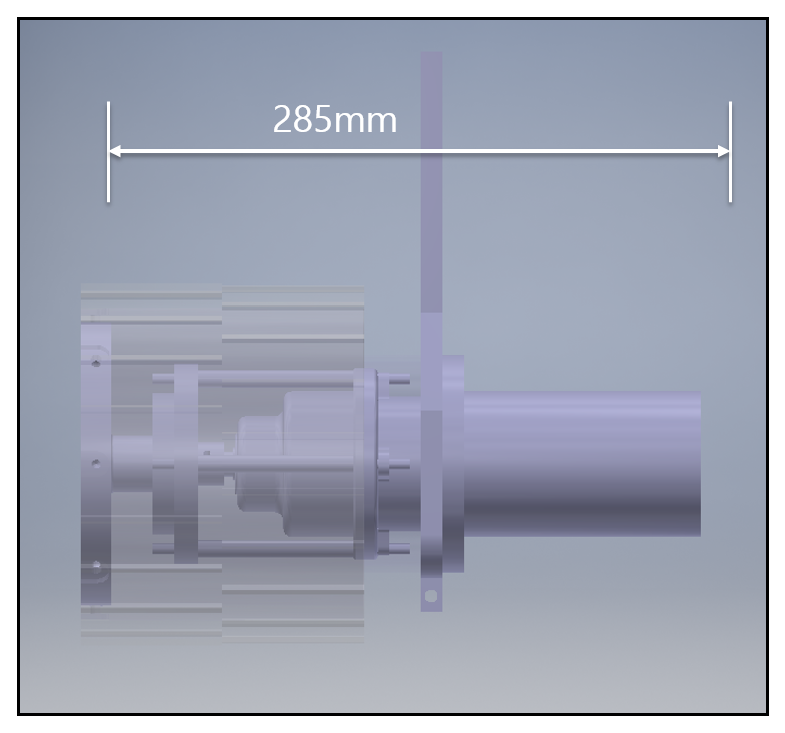
\includegraphics[clip,scale=0.5]{./figure/stac_cad.eps}
		\hspace{1.6cm}
		\end{minipage}

		\begin{minipage}{0.5\hsize}
		\centering
		
\includegraphics[clip,scale=1.0]{./figure/stac_wheel.eps}
		\hspace{1.6cm}
		\end{minipage}

	\end{tabular}	
	\caption{前年度までの駆動モジュールの問題点}
	\label{problem}
\end{figure}

\subsection{研究目的}
\ \ 前述の問題点を考慮し,本研究ではロボットの小型化および構造の簡略化と改善を目的とした.そのための試みとして,ロボットの構造を
\begin{enumerate}
	\item 制御用センターコンピュータ部
	\item 汎用フレーム
	\item 駆動モジュール
\end{enumerate}
の3要素で構成し,各要素について最適化を行った.さらに,森林環境のみならず屋内や平野といった様々な環境に視野を広げるために,2輪・4輪・6輪と組換え可能なモジュール構造を採用し,組換えることで環境に最適なロボットとなるかを確かめた.